\documentclass[11pt,a4paper]{report}
\usepackage[textwidth=37em,vmargin=30mm]{geometry}
\usepackage{calc,xunicode,amsmath,amssymb,paralist,enumitem,tabu,booktabs,datetime2,xeCJK,xeCJKfntef,listings}
\usepackage{tocloft,fancyhdr,tcolorbox,xcolor,graphicx,eso-pic,xltxtra,xelatexemoji}

\newcommand{\envyear}[0]{2025}
\newcommand{\envdatestr}[0]{2025-03-18}
\newcommand{\envfinaldir}[0]{webdb/2025/20250318/final}

\usepackage[hidelinks]{hyperref}
\hypersetup{
    colorlinks=false,
    pdfpagemode=FullScreen,
    pdftitle={Web Digest - \envdatestr}
}

\setlength{\cftbeforechapskip}{10pt}
\renewcommand{\cftchapfont}{\rmfamily\bfseries\large\raggedright}
\setlength{\cftbeforesecskip}{2pt}
\renewcommand{\cftsecfont}{\sffamily\small\raggedright}

\setdefaultleftmargin{2em}{2em}{1em}{1em}{1em}{1em}

\usepackage{xeCJK,xeCJKfntef}
\xeCJKsetup{PunctStyle=plain,RubberPunctSkip=false,CJKglue=\strut\hskip 0pt plus 0.1em minus 0.05em,CJKecglue=\strut\hskip 0.22em plus 0.2em}
\XeTeXlinebreaklocale "zh"
\XeTeXlinebreakskip = 0pt


\setmainfont{Brygada 1918}
\setromanfont{Brygada 1918}
\setsansfont{IBM Plex Sans}
\setmonofont{JetBrains Mono NL}
\setCJKmainfont{Noto Serif CJK SC}
\setCJKromanfont{Noto Serif CJK SC}
\setCJKsansfont{Noto Sans CJK SC}
\setCJKmonofont{Noto Sans CJK SC}

\setlength{\parindent}{0pt}
\setlength{\parskip}{8pt}
\linespread{1.15}

\lstset{
	basicstyle=\ttfamily\footnotesize,
	numbersep=5pt,
	backgroundcolor=\color{black!5},
	showspaces=false,
	showstringspaces=false,
	showtabs=false,
	tabsize=2,
	captionpos=b,
	breaklines=true,
	breakatwhitespace=true,
	breakautoindent=true,
	linewidth=\textwidth
}






\newcommand{\coverpic}[2]{
    % argv: itemurl, authorname
    Cover photo by #2~~(\href{#1}{#1})
}
\newcommand{\makeheader}[0]{
    \begin{titlepage}
        % \newgeometry{hmargin=15mm,tmargin=21mm,bmargin=12mm}
        \begin{center}
            
            \rmfamily\scshape
            \fontspec{BaskervilleF}
            \fontspec{Old Standard}
            \fontsize{59pt}{70pt}\selectfont
            WEB\hfill DIGEST
            
            \vfill
            % \vskip 30pt
            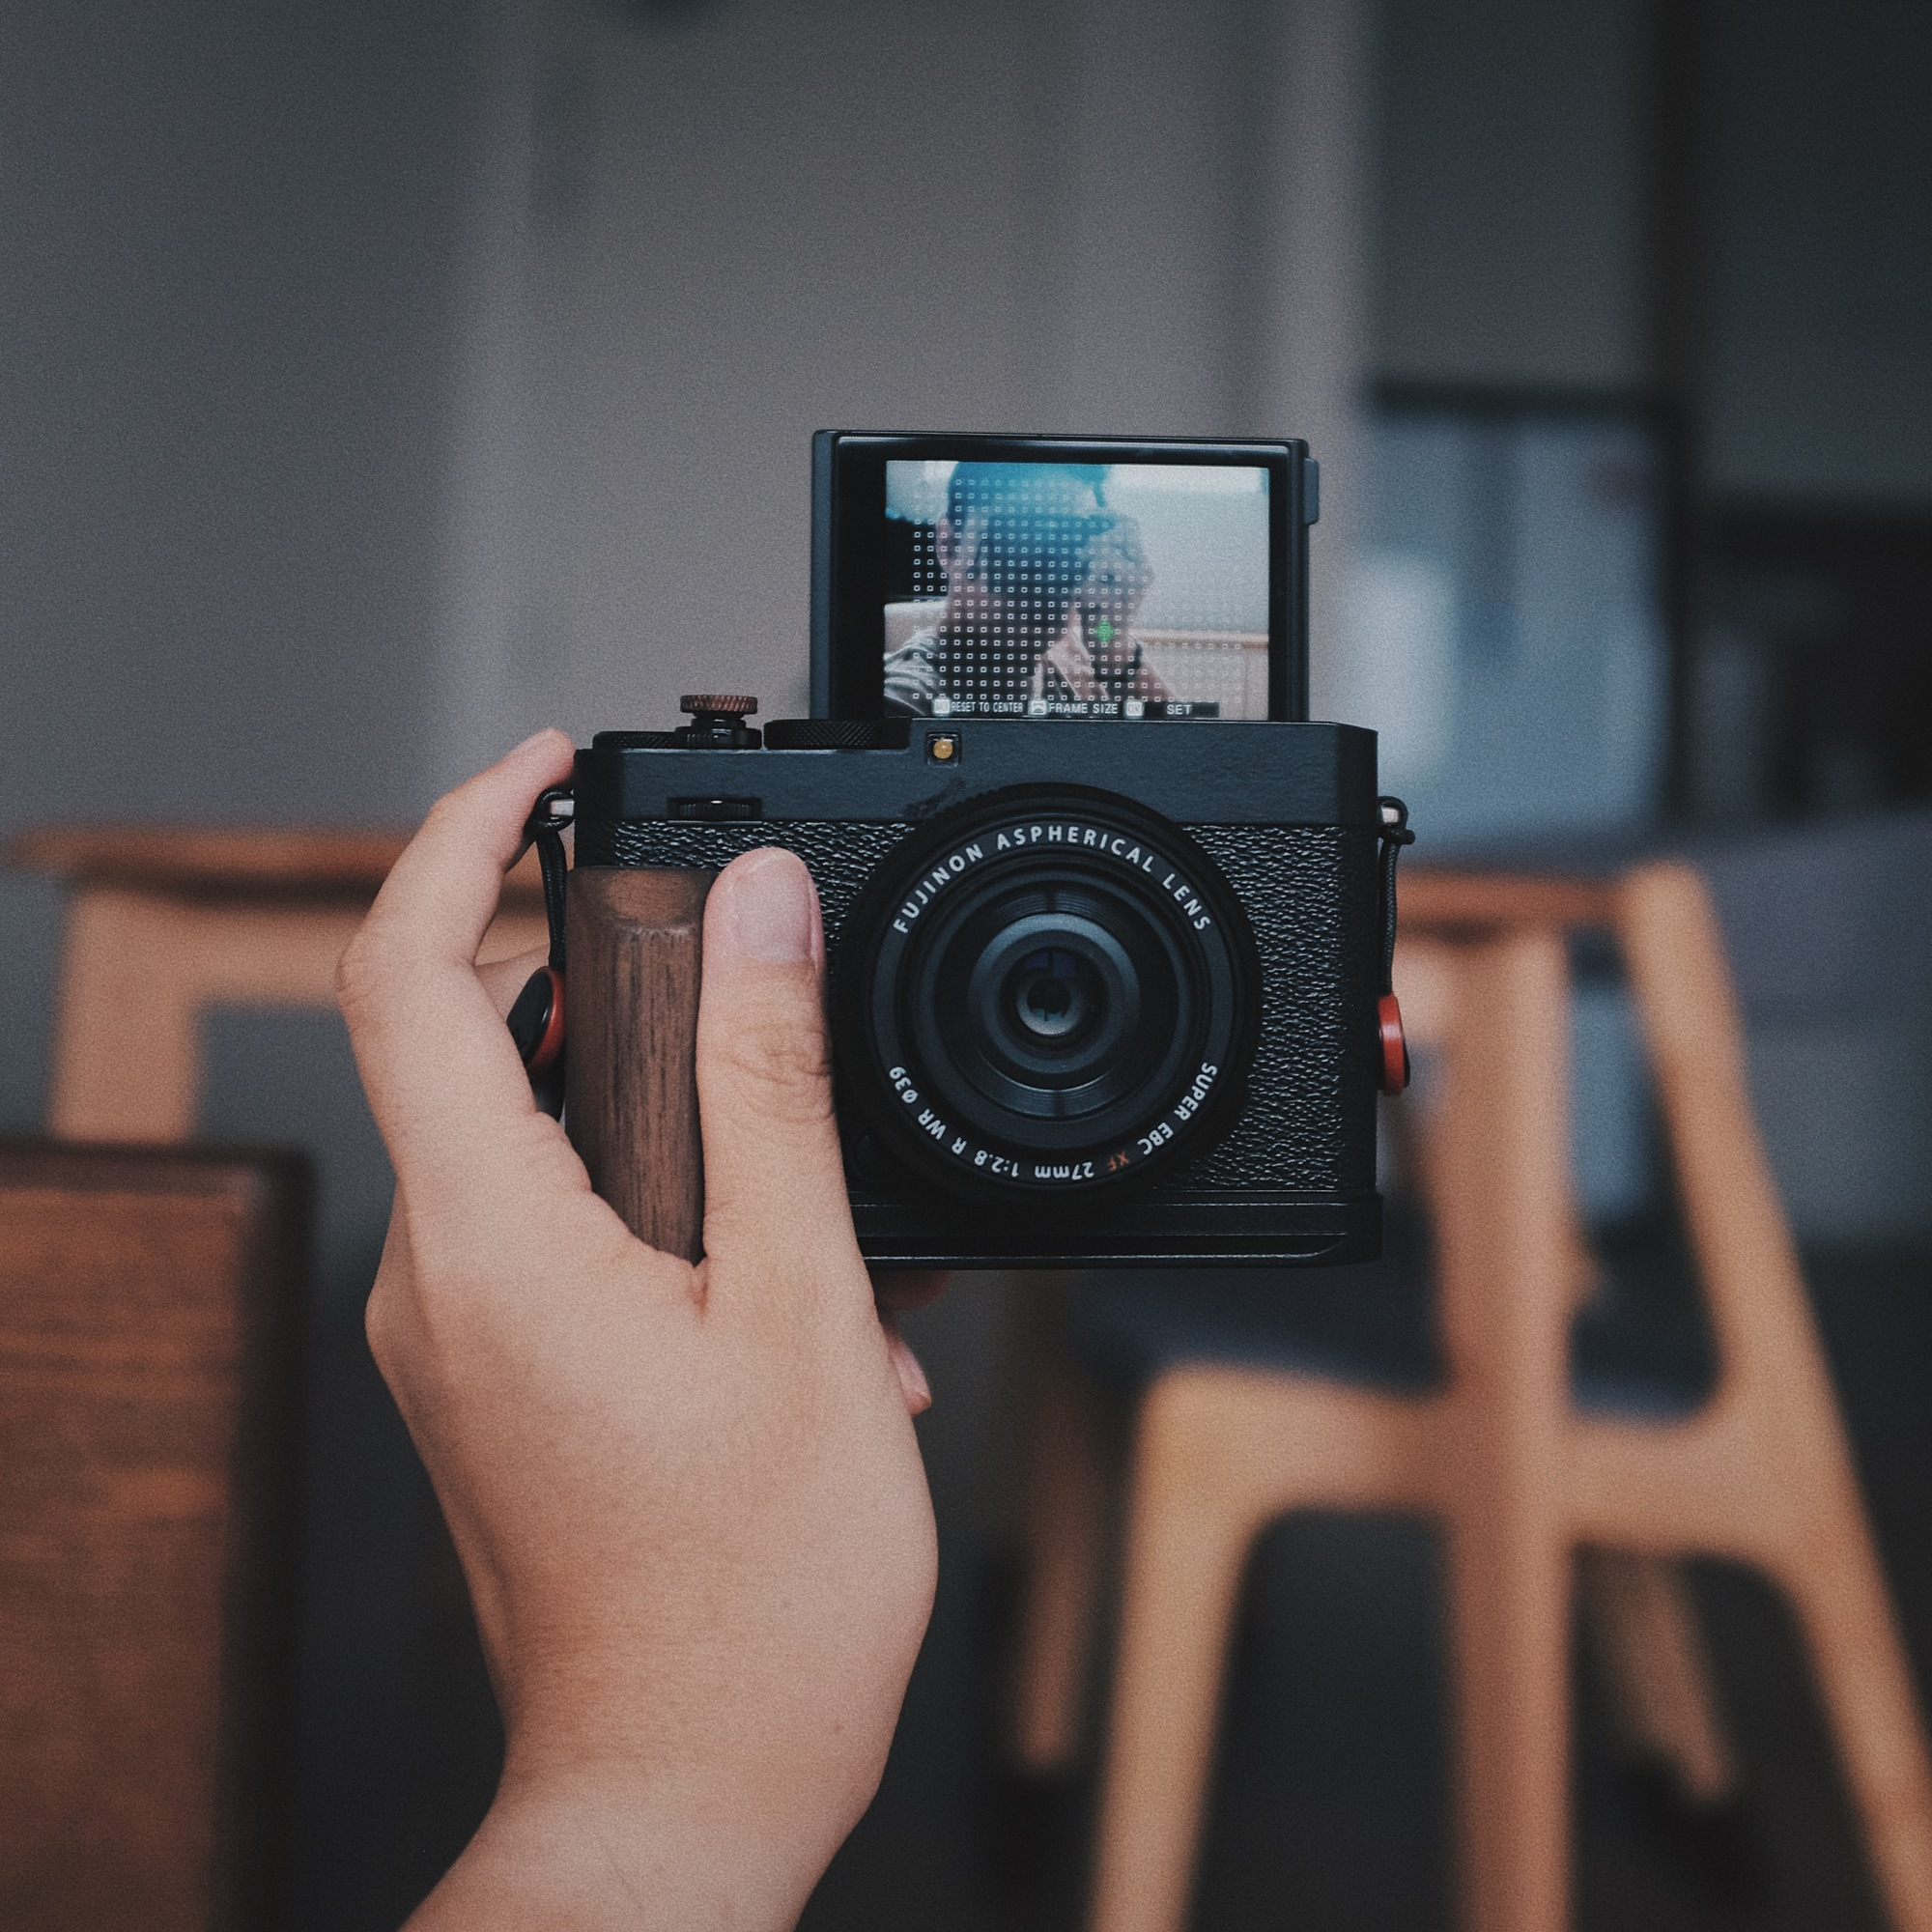
\includegraphics[width=\linewidth]{\envfinaldir/coverpic-prod.jpg}\par
            % \vskip 30pt
            \vfill

            \normalsize\rmfamily\scshape
            \copyright{} The Web Digest Project \hfill\large \envdatestr
        \end{center}
    \end{titlepage}
    % \restoregeometry
}
\newcommand{\simplehref}[1]{%
    \textcolor{blue!80!green}{\href{#1}{#1}}%
}
\renewcommand{\contentsname}{\center\Huge\sffamily\bfseries Contents\par\vskip 20pt}
\newcounter{ipartcounter}
\setcounter{ipartcounter}{0}
\newcommand{\ipart}[1]{
    % \vskip 20pt
    \clearpage
    \stepcounter{ipartcounter}
    \phantomsection
    \addcontentsline{toc}{chapter}{#1}
    % \begin{center}
    %     \Huge
    %     \sffamily\bfseries
    %     #1
    % \end{center}
    % \vskip 20pt plus 7pt
}
\newcounter{ichaptercounter}
\setcounter{ichaptercounter}{0}
\newcommand{\ichapter}[1]{
    % \vskip 20pt
    \clearpage
    \stepcounter{ichaptercounter}
    \phantomsection
    \addcontentsline{toc}{section}{\numberline{\arabic{ichaptercounter}}#1}
    \begin{center}
        \Huge
        \sffamily\bfseries
        #1
    \end{center}
    \vskip 20pt plus 7pt
}
\newcommand{\entrytitlefont}[1]{\subsection*{\raggedright\Large\sffamily\bfseries#1}}
\newcommand{\entryitemGeneric}[2]{
    % argv: title, url
    \parbox{\linewidth}{
        \entrytitlefont{#1}\par\vskip 5pt
        \footnotesize\ttfamily\mdseries
        \simplehref{#2}
    }\vskip 11pt plus 11pt minus 1pt
}
\newcommand{\entryitemGithub}[3]{
    % argv: title, url, desc
    \parbox{\linewidth}{
        \entrytitlefont{#1}\par\vskip 5pt
        \footnotesize\ttfamily\mdseries
        \simplehref{#2}\par\vskip 5pt
        \small\rmfamily\mdseries#3
    }\vskip 11pt plus 11pt minus 1pt
}
\newcommand{\entryitemAp}[3]{
    % argv: title, url, desc
    \parbox{\linewidth}{
        \entrytitlefont{#1}\par\vskip 5pt
        \footnotesize\ttfamily\mdseries
        \simplehref{#2}\par\vskip 5pt
        \small\rmfamily\mdseries#3
    }\vskip 11pt plus 11pt minus 1pt
}
\newcommand{\entryitemHackernews}[3]{
    % argv: title, hnurl, rawurl
    % \parbox{\linewidth}{
    %     \entrytitlefont{#1}\par\vskip 5pt
    %     \footnotesize\ttfamily\mdseries
    %     \simplehref{#3}\par
    %     \textcolor{black!50}{\href{#2}{#2}}
    % }\vskip 11pt plus 11pt minus 1pt
    \begin{minipage}{\linewidth}
            \entrytitlefont{#1}\par\vskip 5pt
            \footnotesize\ttfamily\mdseries
            \simplehref{#3}\par
            \textcolor{black!50}{\href{#2}{#2}}
    \end{minipage}\par\vskip 11pt plus 11pt minus 1pt
}







\begin{document}

\makeheader

\tableofcontents\clearpage




\ipart{Developers}
\ichapter{Hacker News}
\entryitemTwoLinks{GIMP 3.0 Released}{https://news.ycombinator.com/item?id=43393822}{https://testing.gimp.org/news/2025/03/16/gimp-3-0-released/}

\entryitemTwoLinks{Amazon plans to lay off 14,000 managerial positions to save \$3.5B yearly}{https://news.ycombinator.com/item?id=43393079}{https://techstartups.com/2025/03/17/amazon-to-lay-off-14000-managerial-positions-to-save-3-5-billion-annually/}

\entryitemTwoLinks{Archival Storage}{https://news.ycombinator.com/item?id=43391459}{https://blog.dshr.org/2025/03/archival-storage.html}

\entryitemTwoLinks{Dataminr tracked Gaza-related protests}{https://news.ycombinator.com/item?id=43390747}{https://theintercept.com/2025/03/17/lapd-surveillance-gaza-palestine-protests-dataminr/}

\entryitemTwoLinks{Alphabet spins out Taara – Internet over lasers}{https://news.ycombinator.com/item?id=43390467}{https://x.company/blog/posts/taara-graduation/}

\entryitemTwoLinks{Deep Learning Is Not So Mysterious or Different}{https://news.ycombinator.com/item?id=43390400}{https://arxiv.org/abs/2503.02113}

\entryitemTwoLinks{Chaos in the Cloudflare Lisbon Office}{https://news.ycombinator.com/item?id=43389064}{https://blog.cloudflare.com/chaos-in-cloudflare-lisbon-office-securing-the-internet-with-wave-motion/}

\entryitemTwoLinks{Undergraduate Disproves 40-Year-Old Conjecture, Invents New Kind of Hash Table}{https://news.ycombinator.com/item?id=43388296}{https://www.wired.com/story/undergraduate-upends-a-40-year-old-data-science-conjecture/}

\entryitemTwoLinks{Raspberry Pi RP2350 Now Available for Purchase, Stacked Memory Variant Coming}{https://news.ycombinator.com/item?id=43388221}{https://www.phoronix.com/news/Raspberry-Pi-RP2350-Buy}

\entryitemTwoLinks{Rippling Sues Deel over Spying}{https://news.ycombinator.com/item?id=43388133}{https://twitter.com/parkerconrad/status/1901615179718406276}

\entryitemTwoLinks{Meta puts stop on promotion of tell-all book by former employee}{https://news.ycombinator.com/item?id=43387325}{https://www.theguardian.com/technology/2025/mar/13/meta-careless-people-book-former-employee}

\entryitemTwoLinks{Akira ransomware can be cracked with sixteen RTX 4090 GPUs in around ten hours}{https://news.ycombinator.com/item?id=43387188}{https://www.tomshardware.com/tech-industry/cyber-security/akira-ransomware-cracked-with-rtx-4090-new-exploit-to-brute-force-encryption-attack}

\entryitemTwoLinks{Underware 2.0 – Open Source Infinite Cable Management}{https://news.ycombinator.com/item?id=43386578}{https://makerworld.com/en/models/783010-underware-2-0-infinite-cable-management}

\entryitemTwoLinks{uv downloads overtake Poetry for Wagtail users}{https://news.ycombinator.com/item?id=43386357}{https://wagtail.org/blog/uv-overtakes-poetry/}

\entryitemTwoLinks{The exceptional Jordan algebra (2020)}{https://news.ycombinator.com/item?id=43386004}{https://cp4space.hatsya.com/2020/10/28/the-exceptional-jordan-algebra/}

\entryitemTwoLinks{The Alexa feature "do not send voice recordings" you enabled no longer available}{https://news.ycombinator.com/item?id=43385268}{https://discuss.systems/@dev/114161826926246661}

\entryitemTwoLinks{Conducting forensics of mobile devices to find signs of a potential compromise}{https://news.ycombinator.com/item?id=43384894}{https://github.com/mvt-project/mvt}

\entryitemTwoLinks{Genomic study: our capacity for language emerged at least 135k years ago}{https://news.ycombinator.com/item?id=43384826}{https://phys.org/news/2025-03-genomic-capacity-language-emerged-years.html}

\entryitemTwoLinks{Let's knock down social media's walled gardens – Tim Berners-Lee}{https://news.ycombinator.com/item?id=43384786}{https://www.ft.com/content/79d2d19a-08df-48fc-9a6f-a9dbef58f642}

\entryitemTwoLinks{Brown University Professor Is Deported Despite a Judge's Order}{https://news.ycombinator.com/item?id=43384730}{https://www.nytimes.com/2025/03/16/us/brown-university-rasha-alawieh-professor-deported.html}\ichapter{Phoronix}
\entryitemGeneric{\hskip 0pt{}Nginx Rejects Dark Mode Support For Error Pages}{https://www.phoronix.com/news/Nginx-Dark-Mode-Errors-Rejected}

\entryitemGeneric{\hskip 0pt{}Big Rust Update Merged For GCC 15 - Lands The Polonius Borrow Checker}{https://www.phoronix.com/news/GCC-15-Big-GCCRS-Update}

\entryitemGeneric{\hskip 0pt{}AMD Ryzen 9 9900X3D Linux Performance}{https://www.phoronix.com/review/amd-ryzen-9-9900x3d}

\entryitemGeneric{\hskip 0pt{}Intel XeSS SDK 2.0.1 Published With New XeSS 2 Features, Still Closed-Source}{https://www.phoronix.com/news/Intel-XeSS-SDK-2.0.1}

\entryitemGeneric{\hskip 0pt{}Raspberry Pi RP2350 Now Available For Purchase, Stacked Memory Variant Coming Soon}{https://www.phoronix.com/news/Raspberry-Pi-RP2350-Buy}

\entryitemGeneric{\hskip 0pt{}FFmpeg Lands Vulkan Improvements With Initial FFV1 Vulkan Decoder}{https://www.phoronix.com/news/FFmpeg-Vulkan-FFV1}

\entryitemGeneric{\hskip 0pt{}FreeDesktop.org GitLab Begins Its Week Long Cloud/Server Migration}{https://www.phoronix.com/news/FDo-GitLab-Migrate-Begins}

\entryitemGeneric{\hskip 0pt{}Ubuntu 25.04 To Enable NVIDIA Dynamic Boost By Default}{https://www.phoronix.com/news/Ubuntu-25.04-NV-Dynamic-Boost}

\entryitemGeneric{\hskip 0pt{}GIMP 3.0 Stable Being Released As Long-Awaited Update To Adobe Photoshop Alternative}{https://www.phoronix.com/news/GIMP-3.0-Tagged}\ichapter{Dribbble}
\entryitemGeneric{\hskip 0pt{}Abstract S Logo Design // For Sale}{https://dribbble.com/shots/25764643-Abstract-S-Logo-Design-For-Sale}

\entryitemGeneric{\hskip 0pt{}Fintech icons pack part 3 for download}{https://dribbble.com/shots/25728645-Fintech-icons-pack-part-3-for-download}

\entryitemGeneric{\hskip 0pt{}Triceratops}{https://dribbble.com/shots/25761010-Triceratops}

\entryitemGeneric{\hskip 0pt{}Tab Bar Animation}{https://dribbble.com/shots/25760227-Tab-Bar-Animation}

\entryitemGeneric{\hskip 0pt{}Chief Logo Design Process}{https://dribbble.com/shots/25759736-Chief-Logo-Design-Process}

\entryitemGeneric{\hskip 0pt{}World Clock App Design}{https://dribbble.com/shots/25760174-World-Clock-App-Design}

\entryitemGeneric{\hskip 0pt{}Carbon Solutions B2B Dashboard Design}{https://dribbble.com/shots/25681782-Carbon-Solutions-B2B-Dashboard-Design}

\entryitemGeneric{\hskip 0pt{}Bir-D / D.Bird}{https://dribbble.com/shots/25757221-Bir-D-D-Bird}

\entryitemGeneric{\hskip 0pt{}Logowave Awards Entry from Lepisov Branding}{https://dribbble.com/shots/25755190-Logowave-Awards-Entry-from-Lepisov-Branding}

\entryitemGeneric{\hskip 0pt{}Flare - Logo Design 🚀}{https://dribbble.com/shots/25754585-Flare-Logo-Design}

\entryitemGeneric{\hskip 0pt{}Squid Book}{https://dribbble.com/shots/25756273-Squid-Book}

\entryitemGeneric{\hskip 0pt{}Order detail dashboard}{https://dribbble.com/shots/25748173-Order-detail-dashboard}

\entryitemGeneric{\hskip 0pt{}Pricing Plan Web Page Design}{https://dribbble.com/shots/25755045-Pricing-Plan-Web-Page-Design}

\entryitemGeneric{\hskip 0pt{}Bounce}{https://dribbble.com/shots/25755477-Bounce}

\entryitemGeneric{\hskip 0pt{}Fishing Tournament Logo}{https://dribbble.com/shots/25750107-Fishing-Tournament-Logo}

\entryitemGeneric{\hskip 0pt{}Triceratops}{https://dribbble.com/shots/25749787-Triceratops}

\entryitemGeneric{\hskip 0pt{}Lamar® 21°}{https://dribbble.com/shots/25750164-Lamar-21}

\entryitemGeneric{\hskip 0pt{}Sergeant Scooper}{https://dribbble.com/shots/25749566-Sergeant-Scooper}

\entryitemGeneric{\hskip 0pt{}Atoms - Logo Concepts}{https://dribbble.com/shots/25749091-Atoms-Logo-Concepts}

\entryitemGeneric{\hskip 0pt{}Line Icons}{https://dribbble.com/shots/25749882-Line-Icons}

\entryitemGeneric{\hskip 0pt{}Logo For Designed.supply}{https://dribbble.com/shots/25748434-Logo-For-Designed-supply}

\entryitemGeneric{\hskip 0pt{}Codila Studio}{https://dribbble.com/shots/25749456-Codila-Studio}

\entryitemGeneric{\hskip 0pt{}Logo Database (V7) 2024—25}{https://dribbble.com/shots/25743610-Logo-Database-V7-2024-25}

\entryitemGeneric{\hskip 0pt{}Cullet LLC}{https://dribbble.com/shots/25750266-Cullet-LLC}


\ipart{Developers~~~~(zh-Hans)}
\ichapter{Solidot}
\entryitemGeneric{\hskip 0pt{}屏幕时间与心血管病风险上升相关}{https://www.solidot.org/story?sid=80807}

\entryitemGeneric{\hskip 0pt{}Blue Ghost 探测器记录到日全食}{https://www.solidot.org/story?sid=80806}

\entryitemGeneric{\hskip 0pt{}七大科技公司推动中国股市上涨}{https://www.solidot.org/story?sid=80805}

\entryitemGeneric{\hskip 0pt{}中国五岁以下儿童可避免死亡率过去几十年显著下降}{https://www.solidot.org/story?sid=80804}

\entryitemGeneric{\hskip 0pt{}水中有氧运动有助于减肥}{https://www.solidot.org/story?sid=80803}

\entryitemGeneric{\hskip 0pt{}Waymo 的无人出租车去年在旧金山收到了 589 张违反停车规定的罚单}{https://www.solidot.org/story?sid=80802}

\entryitemGeneric{\hskip 0pt{}美国 Z 世代的储蓄不足以支付一个月的开支}{https://www.solidot.org/story?sid=80801}

\entryitemGeneric{\hskip 0pt{}移除对 32 位 PhysX 支持影响英伟达新显卡性能}{https://www.solidot.org/story?sid=80800}

\entryitemGeneric{\hskip 0pt{}开源中国停止招募接收方、再次决定关闭スラド}{https://www.solidot.org/story?sid=80799}

\entryitemGeneric{\hskip 0pt{}空间站太干净不利于宇航员健康}{https://www.solidot.org/story?sid=80798}

\entryitemGeneric{\hskip 0pt{}回顾 Firefox 的分支}{https://www.solidot.org/story?sid=80797}\ichapter{V2EX}
\entryitemGeneric{\hskip 0pt{}[硬件] 请问还有开放接口的监视器或相机}{https://www.v2ex.com/t/1119192}

\entryitemGeneric{\hskip 0pt{}[Apple] Mac Studio 实战 671B 全量大模型成绩出来了}{https://www.v2ex.com/t/1119191}

\entryitemGeneric{\hskip 0pt{}[职场话题] 求指点迷津:老家年到手十万公务员 vs 大厂年包 30w}{https://www.v2ex.com/t/1119189}

\entryitemGeneric{\hskip 0pt{}[远程工作] [广州][外资银行]私有云工程师}{https://www.v2ex.com/t/1119188}

\entryitemGeneric{\hskip 0pt{}[分享发现] 下到木马了,给我浏览器 cookie 全部偷走了}{https://www.v2ex.com/t/1119187}

\entryitemGeneric{\hskip 0pt{}[生活] 给 V 友普法 重点强调 1: 交通事故中,事故责任划分比例不等于事故损失赔偿比例}{https://www.v2ex.com/t/1119186}

\entryitemGeneric{\hskip 0pt{}[程序员] 用 AI 写了一个随机八股文生成器}{https://www.v2ex.com/t/1119185}

\entryitemGeneric{\hskip 0pt{}[分享创造] [TestFlight] Swads - 群晖 Download Station 客户端}{https://www.v2ex.com/t/1119184}

\entryitemGeneric{\hskip 0pt{}[生活] 借 V 站替姐姐相亲一下,走过路过别错过。}{https://www.v2ex.com/t/1119183}

\entryitemGeneric{\hskip 0pt{}[职场话题] 人就必须一直工作吗?因为两年前的空窗期反手被拒了}{https://www.v2ex.com/t/1119182}

\entryitemGeneric{\hskip 0pt{}[买买买] 各位帥哥 想找一款 4k 高刷, usb hub 顯示器 有推薦嗎}{https://www.v2ex.com/t/1119181}

\entryitemGeneric{\hskip 0pt{}[MacBook] macbook 扩容硬盘,如何找靠谱的店铺}{https://www.v2ex.com/t/1119180}

\entryitemGeneric{\hskip 0pt{}[酷工作] [杭州] 总包 50-60w / 基础平台工程师 / 2-6 年经验 / Kubernetes DevOps / 直招}{https://www.v2ex.com/t/1119179}

\entryitemGeneric{\hskip 0pt{}[问与答] 你们愿意为什么程度的 AI 功能付费呢?}{https://www.v2ex.com/t/1119178}

\entryitemGeneric{\hskip 0pt{}[git] 推送远程仓库导致本地提交记录消失,如何找回}{https://www.v2ex.com/t/1119177}

\entryitemGeneric{\hskip 0pt{}[iPhone] iPhone 16 pro 各组件 应该选 哪个厂家?}{https://www.v2ex.com/t/1119176}

\entryitemGeneric{\hskip 0pt{}[问与答] asus zenfone 9 android 14 无法设置勿扰模式的时长?}{https://www.v2ex.com/t/1119175}

\entryitemGeneric{\hskip 0pt{}[分享创造] 分享一下最近我使用 AI 创作的 2 个网站。}{https://www.v2ex.com/t/1119174}

\entryitemGeneric{\hskip 0pt{}[JavaScript] 记忆中好像在论坛看到有款专门在 iframe 中做前端的 js 库/框架?}{https://www.v2ex.com/t/1119172}

\entryitemGeneric{\hskip 0pt{}[Android] 为什么在 Linux 下构建 APK 比用 Windows 快非常多}{https://www.v2ex.com/t/1119171}

\entryitemGeneric{\hskip 0pt{}[MacBook Air] 新入 MBA 丐版,有什么办法破除 256g 硬盘焦虑?}{https://www.v2ex.com/t/1119169}

\entryitemGeneric{\hskip 0pt{}[Apple] Mac mini / MacBook Air 教育优惠叠加国补}{https://www.v2ex.com/t/1119168}

\entryitemGeneric{\hskip 0pt{}[Apple] iPhone 16 Pro,设置了充电上限 80\%,有时候还是会充到 100\%是怎么回事?}{https://www.v2ex.com/t/1119167}

\entryitemGeneric{\hskip 0pt{}[职场话题] Java 春招,求大佬指点迷津}{https://www.v2ex.com/t/1119166}

\entryitemGeneric{\hskip 0pt{}[分享创造] EditorJumper: 让 Cursor、VS Code、trae、Windsurf 和 JetBrains IDE 切换如丝般顺滑}{https://www.v2ex.com/t/1119165}

\entryitemGeneric{\hskip 0pt{}[分享发现] Gitlab 不对大陆服务了,要删号了}{https://www.v2ex.com/t/1119163}

\entryitemGeneric{\hskip 0pt{}[酷工作] [广州] C++推荐\&大模型推理优化方向}{https://www.v2ex.com/t/1119162}

\entryitemGeneric{\hskip 0pt{}[汽车] 比亚迪发布的这个兆瓦闪充怎么看}{https://www.v2ex.com/t/1119161}

\entryitemGeneric{\hskip 0pt{}[分享创造] 我开发了一个在线加密网站 localfileencrypt.com,在本地使用 AES-256 加密您的文本/文件/文件夹,欢迎体验~}{https://www.v2ex.com/t/1119160}

\entryitemGeneric{\hskip 0pt{}[程序员] manus 比我想的要强}{https://www.v2ex.com/t/1119159}

\entryitemGeneric{\hskip 0pt{}[酷工作] [快手] [内推] 商业化技术各方向、低中高级别均有 hc}{https://www.v2ex.com/t/1119158}

\entryitemGeneric{\hskip 0pt{}[Mac mini] 有推荐用于 mini m4 的 4k 显示器吗}{https://www.v2ex.com/t/1119156}

\entryitemGeneric{\hskip 0pt{}[VXNA] 申请收录个人博客: 从不说安全词}{https://www.v2ex.com/t/1119153}

\entryitemGeneric{\hskip 0pt{}[Vue.js] 使用 Ant design X vue 组件库怎么解决无法正确展示 MarkDown 格式字符串的问题?}{https://www.v2ex.com/t/1119152}

\entryitemGeneric{\hskip 0pt{}[OpenAI] 请问数据多,可以做数据分析吗}{https://www.v2ex.com/t/1119151}

\entryitemGeneric{\hskip 0pt{}[问与答] 想给一个高一学生送生日礼物,想让他了解目前最前沿的科技,有什么推荐?预算在 2 万元人民币以内,特别有意义的可以突破预算。}{https://www.v2ex.com/t/1119150}

\entryitemGeneric{\hskip 0pt{}[酷工作] Hot/New Jobs: 高级 Java 技术专家 大数据开发}{https://www.v2ex.com/t/1119149}

\entryitemGeneric{\hskip 0pt{}[酷工作] 上过央视的杭州机器人公司招 Linux C++ 应用软件工程师}{https://www.v2ex.com/t/1119148}

\entryitemGeneric{\hskip 0pt{}[Apple] 建议各位 Mac 用户在买显示器时考虑高刷屏}{https://www.v2ex.com/t/1119147}

\entryitemGeneric{\hskip 0pt{}[前端开发] 2025 年了,flutter 还是 react}{https://www.v2ex.com/t/1119146}

\entryitemGeneric{\hskip 0pt{}[电影] 有看过《万能钥匙》的么}{https://www.v2ex.com/t/1119145}

\entryitemGeneric{\hskip 0pt{}[问与答] 国内有哪些做代理 ip 比较稳定价格实惠的?看到一家厉害的 oxylabs 有点贵}{https://www.v2ex.com/t/1119143}

\entryitemGeneric{\hskip 0pt{}[微软] Office 365 账号求助。}{https://www.v2ex.com/t/1119142}

\entryitemGeneric{\hskip 0pt{}[职场话题] 复试说是部门负责人,等了好几天,结果进来一个产品交叉面试说是}{https://www.v2ex.com/t/1119140}

\entryitemGeneric{\hskip 0pt{}[Apple] AppleCare+ 的一点误解}{https://www.v2ex.com/t/1119139}

\entryitemGeneric{\hskip 0pt{}[问与答] 国内科技大厂的综合实力和美国同行比到底是强还弱?}{https://www.v2ex.com/t/1119138}

\entryitemGeneric{\hskip 0pt{}[macOS] AirPods 降噪 快捷指令无法在 sequoia 系统上运行}{https://www.v2ex.com/t/1119136}

\entryitemGeneric{\hskip 0pt{}[求职] 8 年经验 PHP 求个远程岗位}{https://www.v2ex.com/t/1119135}

\entryitemGeneric{\hskip 0pt{}[分享创造] 完全免费的 AI 生成图片网站,蹲一个蹲}{https://www.v2ex.com/t/1119134}

\entryitemGeneric{\hskip 0pt{}[香港] 人在香港开户,有邀请的发过来...}{https://www.v2ex.com/t/1119133}


\ipart{Generic News}
\ichapter{Reuters}
\entryitemWithDescription{\hskip 0pt{}Russia close to ejecting Ukrainian forces from Kursk, Kremlin says}{https://www.reuters.com/world/europe/russia-close-ejecting-ukrainian-forces-kursk-kremlin-says-2025-03-13/}{Russia\textquotesingle s operation to eject Ukrainian forces from the western Russian of Kursk has entered its final stage, state news agency TASS reported on Thursday citing Kremlin spokesman Dmitry...}

\entryitemWithDescription{\hskip 0pt{}Turkey could be a vital partner as Europe, Ukraine seek new security framework}{https://www.reuters.com/world/europe/turkey-could-be-vital-partner-europe-ukraine-seek-new-security-framework-2025-03-13/}{Turkey has emerged as a key potential partner in restructuring European security, diplomats and analysts say, as Europe scrambles to bolster its defence and find guarantees for Ukraine under any forthcoming ceasefire deal urged by the...}

\entryitemWithDescription{\hskip 0pt{}Canada announces plan to ease Syria sanctions}{https://www.reuters.com/world/canada-announces-plan-ease-syria-sanctions-2025-03-13/}{The Canadian government on Wednesday announced plans to ease sanctions on Syria during what it called a period of...}

\entryitemWithDescription{\hskip 0pt{}G7 foreign ministers meet in Canada amid tensions with Trump}{https://www.reuters.com/world/g7-foreign-ministers-meet-canada-amid-tensions-with-trump-2025-03-13/}{Foreign ministers of leading Western democracies meet in Canada on Thursday after seven weeks of rising tensions between U.S. allies and President Donald Trump over his upending of foreign policy on Ukraine and imposing of...}

\entryitemWithDescription{\hskip 0pt{}Pakistan train hijack hostages end ordeal with arrival in Quetta}{https://www.reuters.com/world/asia-pacific/pakistan-train-hijack-hostages-end-ordeal-with-arrival-quetta-2025-03-13/}{Dozens of people rescued from a train hijacked by separatist militants in southwest Pakistan arrived on Thursday in the city of Quetta, hours after security forces killed all 33 attackers to end a day-long...}

\entryitemWithDescription{\hskip 0pt{}China accuses New Zealand's top spy of spreading 'false information'}{https://www.reuters.com/world/asia-pacific/china-accuses-new-zealands-top-spy-spreading-false-information-2025-03-13/}{China\textquotesingle s embassy in New Zealand on Thursday accused Wellington\textquotesingle s top spy of "spreading false information" after the intelligence chief warned of security risks posed by Beijing\textquotesingle s growing...}

\entryitemWithDescription{\hskip 0pt{}Duterte takes responsibility for Philippines drug war, anticipates long ICC battle}{https://www.reuters.com/world/asia-pacific/duterte-takes-responsibility-philippines-drug-war-anticipates-long-icc-battle-2025-03-13/}{Former Philippine President Rodrigo Duterte said he takes full responsibility for his administration\textquotesingle s "war on drugs", in a video message posted on his Facebook account, as he braces for a legal battle at the International...}

\entryitemWithDescription{\hskip 0pt{}US Justice Department investigating New York migrant hotels, reports say}{https://www.reuters.com/world/us/us-justice-department-investigating-new-york-migrant-hotels-reports-say-2025-03-13/}{The U.S. Justice Department on Wednesday opened an investigation into the operation of New York City hotels as migrant shelters, according to media...}

\entryitemWithDescription{\hskip 0pt{}South Korea charges air force pilots with criminal negligence in accidental bombing of village}{https://www.reuters.com/world/asia-pacific/south-korea-charges-air-force-pilots-with-criminal-negligence-accidental-bombing-2025-03-13/}{South Korean military investigators charged two Air Force pilots on Thursday with criminal negligence over an accidental bombing of a village last week during a training exercise, which injured at least 29 people and caused extensive...}

\entryitemWithDescription{\hskip 0pt{}Russia lays out demands for talks with US on Ukraine, sources say}{https://www.reuters.com/world/europe/russia-lays-out-demands-talks-with-us-ukraine-sources-say-2025-03-13/}{Russia has presented the U.S. with a list of demands for a deal to end its war against Ukraine and reset relations with Washington, according to two people familiar with the...}

\entryitemWithDescription{\hskip 0pt{}Exclusive: Wife of detained Palestinian Columbia student says she was naive to believe he was safe from arrest}{https://www.reuters.com/world/us/wife-arrested-columbia-student-says-she-was-naive-believe-he-was-secure-2025-03-12/}{Two days before U.S. agents arrested Mahmoud Khalil, the Columbia University student and Palestinian activist asked his wife if she knew what to do if immigration agents came to their...}

\entryitemWithDescription{\hskip 0pt{}Mark Carney to be sworn in as Canada's prime minister on Friday}{https://www.reuters.com/world/americas/mark-carney-be-sworn-canadas-prime-minister-friday-media-reports-2025-03-12/}{Mark Carney will be sworn in as Canada\textquotesingle s next prime minister on Friday morning, marking the final day of Justin Trudeau\textquotesingle s more than nine years in...}

\entryitemWithDescription{\hskip 0pt{}NASA, SpaceX delay flight that was to retrieve stuck astronauts}{https://www.reuters.com/technology/space/spacex-nasa-set-astronaut-flight-that-will-retrieve-stuck-astronauts-2025-03-12/}{NASA and SpaceX on Wednesday delayed the launch of a replacement crew of four astronauts to the International Space Station that would have set in motion the long-awaited homecoming of U.S. astronauts Butch Wilmore and Suni...}






\clearpage
\leavevmode\vfill
\footnotesize

Copyright \copyright{} 2023-2025 Neruthes and other contributors.

This document is published with CC BY-NC-ND 4.0 license.

The entries listed in this newsletter may be copyrighted by their respective creators.

This newsletter is generated by the Web Digest project.

The newsletters are also delivered via Telegram channel \CJKunderline{\href{https://t.me/webdigestchannel}{https://t.me/webdigestchannel}}.\\
RSS feed is available at \CJKunderline{\href{https://webdigest.pages.dev/rss.xml}{https://webdigest.pages.dev/rss.xml}}.

This newsletter is available in PDF at
\CJKunderline{\href{https://webdigest.pages.dev/}{https://webdigest.pages.dev/}}.

The source code being used to generate this newsletter is available at\\
\CJKunderline{\href{https://github.com/neruthes/webdigest}{https://github.com/neruthes/webdigest}}.

This newsletter is also available in
\CJKunderline{\href{http://webdigest.pages.dev/readhtml/\envyear/WebDigest-20250318.html}{HTML}} and
\CJKunderline{\href{https://github.com/neruthes/webdigest/blob/master/markdown/\envyear/WebDigest-20250318.md}{Markdown}}.


\coverpic{https://unsplash.com/photos/couple-shares-a-kiss-as-the-sun-sets-L0-ig2WymkY}{Alexander Mass}


\end{document}
